\chapter{方案设计与实现}
\label{chap:design}
%Overview
本章重点介绍底层平台感知的高性能NFV平台Furion系统设计。在Furion的设计中,当系统初始化时,将动态性能测试的结果作为运行时参数输入系统,后续算法将以该参数作为算法执行时的参照标准。当系统收到一个服务链的请求后,需要根据当前可用的系统资源余量进行判断是否响应,并将上层抽象的业务需求转化为具体的服务链业务链表,系统的映射模块根据服务链的逻辑链表来映射相应的具体实例。在映射实例的过程中,本系统的原型平台使用的是随机映射的策略,而这种策略在实际的运行环境中缺乏对服务链中所涉及的虚拟机和所分配的底层资源的感知,本设计通过对底层物理资源建模并针对性的提出基于资源亲和度的映射策略,从而提升资源的利用效率和网络服务的性能。

\section{总体设计概述}
\subsection{总体设计目标}
数据从一个网络功能节点传输到另一个节点的过程中不可避免的会产生数据处理和传输的延迟,同时物理带宽同样限制着服务理论带宽上限。在标准的工业生产环境中,单个处理器节点中的物理核数量和内存空间也是有限的,同时通用服务器上不平衡的负载分布也会导致剧烈的资源竞争甚至导致意想不到的性能下降。因此,本文所设计的系统需要相对优化的NFV资源映射和调度策略。在本文中,设计主要关注以下的三个目标:
\begin{enumerate}
	\item 物理资源的实际带宽应当满足服务链的最小带宽需求。
	\item 物理资源的数据传输延迟应当小于服务所允许的最大延迟要求。
	\item 物理资源的整体利用率应当得到保证。一个有效的资源映射策略应当可以保证尽可能的使用可用的物理资源,并在相同的物理资源的前提下提升服务的性能。
\end{enumerate}

\subsection{总体设计思路}
鉴于已有验证性实验的观测结论和以上对此类问题的目标分析,本文所设计的系统需要获取实际服务链的具体组成结构,并考虑具体实例之间物理资源的亲和性来满足实际NFV应用的最小带宽和最大延迟要求,同时在保证服务质量的前提下提升物理资源的整体利用率。

为了实现以上的设计目的,本系统提供了一种基于底层多核运行平台架构感知的虚拟化网络功能的映射方法。在本系统的设计结构中,当Clearwater平台接受到一个服务请求时,会根据服务请求的解析调度虚拟机资源来组织服务链并提供服务。本系统会评估当前服务资源是否满足提供服务的最小需求,即组成服务链的不同功能域中是否有足够的运行实例。当资源充足时,系统开始根据服务链的实际服务数据流转发图来组织服务。在挑选具体服务实例时组成具体SFC时,系统根据预先处理生成的物理资源亲和度矩阵作为调度算法的输入,根据矩阵中每种资源的亲和度大小关系,依照SFC链的连接顺序,使用局部最优的方法搜索构造出最优的服务链与实例的映射关系,最终结果则交由实际映射模块去从虚拟机角度来实现。

从整体架构上分析,实现基于底层多核运行平台的架构感知的虚拟机化网络功能的映射方法,即本文中所设计动态映射系统包括以下关键步骤:

步骤1、对底层平台进行预处理,获得与平台底层运行时相关的信息矩阵。与普通从硬件中读取参数不同,通过动态采样的方法获取平台运行时实时性能参数能更加准确地反映底层平台的架构差异以及所引起的性能差异。首先,动态采样可以实现与操作系统无关性能信息获取,不管多核平台运行的操作系统版本如何,都可以通过采样程序获取该操作系统下的实时运行结果。其次,相比于直接从主板芯片中读取多核架构中不同处理器节点的亲和度信息,动态采样的方法通过动态地运行测试程序,可以获得更加接近实际情况的量化数据。基于这样的数据信息,可以更加准确地刻画底层物理资源之间的细粒度的亲和度信息。最终信息被存进格式化的信息矩阵中,作为步骤2的输入。 

步骤2、当一条服务请求到来时,分析该请求所对应的服务链。根据请求所对应服务链的数据流向确定所需要的虚拟网络功能服务点,使用基于贪心的方法并依照信息矩阵中的参数生成映射决策序列来确定待映射的具体运行实例,进入步骤3。

步骤3、根据步骤2生成映射的实例序列,依次检查实例在对应的物理资源节点当前的负载情况,如果某一实例所在节点的负载过高,增加负载会加剧资源竞争导致当前运行实例的性能下降,则返回步骤2将本次的映射序列标记为失效,重新生成新的实例映射序列。检查通过后进入步骤4。

步骤4、根据生成的映射序列,更新默认的随机选取策略,实现服务链到实际物理资源的映射服务。

步骤5、当服务链服务生命周期结束时,重置服务实例状态为待机中,释放实例资源。

\subsection{总体设计架构}
基于对现有平台默认映射策略不足的研究和分析,本文设计了一套底层运行平台感知的高性能NFV系统,该系统架构如图 \ref{fig:system} 所示,想比于原来的服务链映射方式,本文添加了三个模块来实现前文中的设计目标,即底层信息采样模块(Hardware Prober),服务链分析模块(Service Translator) 和动态协调模块(Dynamic Coordinator)。从图 \ref{fig:system} 中可以看出,本文所设计的系统类似一个中间件方式插入到已有的IMS服务和底层的虚拟化平台之中。上层的业务系统根据具体业务发出服务链服务请求,由管理系统将服务请求下发,服务链需求分析模块收到服务请求后负责根据具体业务给出对应的服务链,形成组网链表并传递到动态协调模块中。动态协调模块收到服务链表后,负责根据底层信息采样模块预先生成的信息矩阵和预设的映射算法生成映射策略。
\begin{figure}[!htp]
	\label{fig:system}
	\centering
	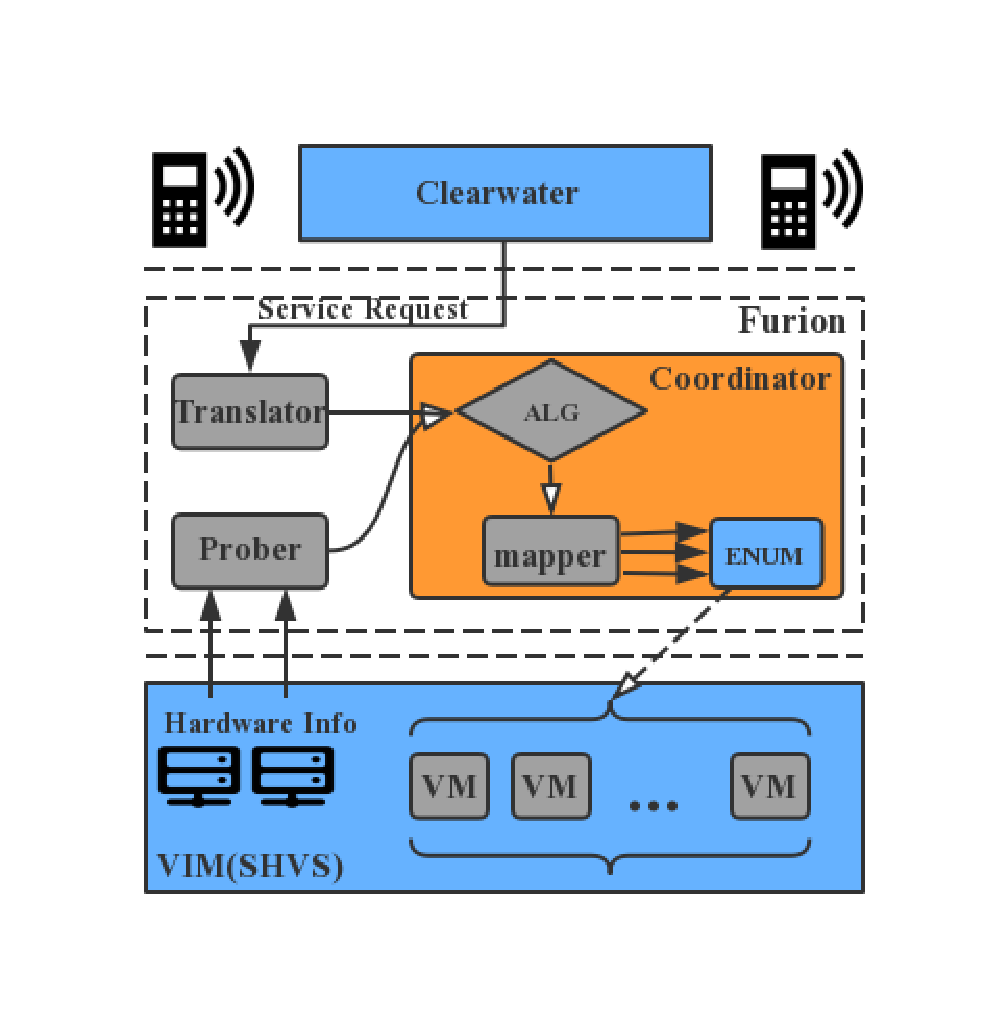
\includegraphics[width=0.8\textwidth]{system.pdf}
	\bicaption[fig:system]{系统架构示意图}{系统架构示意图}{Fig}{System Overview}
\end{figure}

\section{具体模块设计分析}
%TODO 丰富内容和细节
\subsubsection{底层信息采样模块}
如系统架构示意图\ref{fig:system}所示,底层信息采样模块负责从底层硬件获取运行平台架构信息和运行时各节点细粒度的性能信息。通过预处理采样等手段,该模块将获取的硬件信息以信息矩阵的方式存储下来做系统输入。该模块还负责对运行平台进行实时的监控和信息反馈,作为动态映射模块的实时输入参数。在矩阵 $D$ 中,元素 $D_{ij}$ 表示当使用第 $i$ 号访问在位于 $j$ 的资源时,所需要的性能开销。

$$
M =
\begin{pmatrix}
10      & 8      & \cdots & 4      \\
9      & 10      & \cdots & 5      \\
\vdots & \vdots & \ddots & \vdots \\
4      & 3      & \cdots & 10     \\
\end{pmatrix}
$$



\subsubsection{服务链分析模块}
该模块负责在运行时获取并解析上层业务的具体服务请求,将服务请求转化为特定的服务链链表传递给动态映射模块。当特定的服务链链表生成之后,该模块会检查当前运行系统中的资源余量来确定是否响应服务请求。


\subsubsection{动态映射模块}
本文的高性能优化系统基于现有的NFV应用平台 Clearwater 来实现。Clearwater的具体架构与模块相关介绍参见第 \ref{intro:clearwater} 章。在语音和多媒体业务的具体实现中,Clearwater利用云计算资源池化的优势,将各关键网络功能节点以资源池的形式部署在云计算环境中,使用域名解析服务来管理各功能节点之间的连接。默认的服务链实例映射使用随机选取的策略,即根据已有的资源随机选择参与服务组链的运行实例。这样的服务链映射方式随便生成方便管理简单,但是完全忽略了服务链链式服务的数据传输特性,也完全没有考虑底层运行平台的架构差异和资源亲和度信息。同时如果个别处理节点出现负载过高的情况,原有的策略也没有有效的解决方法,甚至有可能加剧某个节点资源竞争,导致服务性能下降的后果。

基于现有的NFV服务平台,本文利用域名解析实现逻辑服务链到实际链路的映射。当动态映射模块收到服务链分析模块传来的特定服务链链表之后,会根据本文提出的基于贪心的算法来生成与逻辑服务链链表相对应的具体实例链表。这里,本文会根据具体实例所在处理节点的实际负载来确定是否重新生成策略。

\section{本章小结}
本章主要介绍了底层平台感知的NFV平台实现方法的设计结构,包括基于服务链的分析建模和本设计的设计目标、设计思路以及详细的模块设计分析。与其他的设计不同,本文从服务链和底层资源的角度出发,进行了相关信息的分析和建模,将物理机的底层资源根据彼此之间的亲和度关系划分为了不同的等价类,并从上层应用的运行实例的角度出发定义了不同物理资源前提下的应用运行所需的成本和随之带来的开销。在所建立模型的基础上,本文提出了设计的所关注的三个目标,并以这些目标作为约束详细阐述了本文的总体设计思路和模块的设计细节。

\chapter{方案实现}
\label{chapter:implement}
本章重点介绍了底层感知的高性能NFV平台的具体实现。本文中,设计方案的原型的实现是在Clearwater应用框架的基础进行的。Clearwater是成熟的商用语音多媒体子系统业务框架之一。由于Clearwater在开源平台Github上开源了其所有代码,任何人可以轻易的获取并在手中的大容量标准通用服务器上部署这项多媒体语音子系统。因此,本系统的原型实现也选择在Clearwater平台上实现。值得指出的是,虽然本系统的实现是基于ClearWater的,但是本设计中的核心设计思想和设计架构具有比较广泛的适用性,也可以适用于其他NFV业务平台。本设计使用非侵入的插入中间件方式实现,没有对业务系统有任何更改,也就是说本设计也能够扩展到其他的NFV业务中,具有一定的可扩展性。
\section{底层信息采样模块}
本文使用经典的内存访问测试工具Stream\footnote{https://www.cs.virginia.edu/stream/} 和Intel Memory Latency Checker\footnote{https://software.intel.com/en-us/articles/intelr-memory-latency-checker} 作为采样工具,预先运行并获取所有运行时参数,作归一化处理分别后存入如下的矩阵中。本文所使用的平台有32个物理核,即可以得到两个32x32的矩阵。所生成的信息参考矩阵被以文件的形式存储在系统硬盘上,随时供其他模块读取。

除了预处理的采样信息,底层信息采样模块包括一个动态的节点负载的监测工具,通过加载系统msr模块来使用PCM工具动态的监测每个物理核当期的负载信息,监测模块每秒更新,将结果输出至文件中。本文中重点关注如表格 \ref{tab:dynamic} 中所列出的信息,其中L3 cache的命中率可作为当前处理器节点的负载参考指标而L2 Cache的命中率可以作为当前物理CPU的负载参考。

\begin{table}[!htb]
	\centering
	\bicaption[tab:dynamic]{服务器实时监测参数}{服务器实时监测参数}{Table}{Table of State Parameters of Running Server}
	\begin{tabular}{ | l | p{6cm} |}\hline
		\textbf{参数} &							 \textbf{参数涵义}  				\\ 	\hline
		IPC   & 当前CPU周期指令数\\ \hline
		L3MISS & L3 cache未命中次数\\ \hline
		L2MISS & L2 cache未命中次数\\ \hline
		L3HIT & L3 cache 命中率 (0.00-1.00)\\ \hline
		L2HIT & L2 cache 命中率 (0.00-1.00)\\ \hline
		L3MPI & 每个指令周期内的L3cache miss数\\ \hline
		L2MPI & 每个指令周期内的L2cache miss数\\ \hline
		READ  & 内存读取数 (GBytes)\\ \hline
		WRITE & 内存写入数 (in GBytes)\\ \hline
	\end{tabular}
\end{table}


\section{服务链分析模块}
服务链分析模块主要负责业务接口,根据上层服务的具体需求来选择选择具体组链方式生成逻辑的服务链链表。这里针对Clearwater的具体业务总结了主要业务流程和所需的服务链请求。业务流程主要包括:用户注册流程,初始化拨号流程,通话流程,和通话终止流程。每个流程的具体流程如图 \ref{fig:flow_register} 到图 \ref{fig:flow_terminate} 所示。根据所总结的服务流程和对应的服务链,本文将每个服务链以链表的形式记录下来存储到预定义的配置文件中。当收到某一类服务请求时,服务链分析模块根据服务请求类型在预定义的文件中选择对应的服务链链表,完成服务链服务分析。具体的服务流程如下:

%TODO 详细叙述流程过程
\textbf{用户注册流程}如图 \ref{fig:flow_register} 所示,主要涉及到的网络功能节点为Sprout和Homestead。当客户端发起注册请求时,Sprout节点将从Homestead节点中获取认证信息,如果没有相关认证记录则请求拒绝, Sprout节点同时缓存该请求记录,一旦后续出现相同请求则直接处理不再查询。如果查询到相关认证记录认证通过,则向客户端返回认证成功。如果有第三方认证,则跳转到第三方登记流程。

\textbf{初始化拨号流程}如图 \ref{fig:flow_dialog}和图 \ref{fig:flow_dialog2} 所示,主要参与的网络功能有Sprout、Homestead当客户端向Sprout节点发起通话请求,Sprout节点通过HTTP请求从Homestead节点缓存中获取拨号者和被拨号信息,同时生成本次服务的iFC\footnote{http://www.3gpp.org/ftp/Specs/archive/29\_series/29.228/29228-b70.zip appendices B and F}。随后Sprout向ENUM组件中查询所拨打用户是否在线,如果在线则Sprout完成查询终止iFC,并根据查询结果向被拨打者发起SIP INVITE请求,同时向AS(Vellum)中记录SIP Ringing状态。当被拨叫客户端接听后,返回SIP 200 OK,则通过Sprout节点更新AS(Vellum)记录。

\textbf{通话流程}如图\ref{fig:flow_inDialog}所示,客户端通过Sprout不断在通话过程中不断更新状态信息到AS(Vellum)中,更新数据同样通过Sprout反馈到被叫客户端中。

\textbf{通话终止流程}如如图\ref{fig:flow_terminate}所示,当通话结束,客户端发起挂断请求,Sprout将状态存储到AS(Vellum)中,并向被拨号者发起SIP BYE请求,请求响应后同样更新AS(Vellum)记录,返回SIP 200 OK,通话终止。

\newpage
%TODO 加入ENUM模块修改方法
\section{动态映射模块}
%TODO 动态映射算法具体实现
在该模块中,本设计将需要根据服务链分析模块中生成的服务链组织链表通过算法 \ref{alg:greedy} 映射成为具体的实例链表,并根据实例链表完成服务链的组件。具体来说,在初始化阶段将所有的实例具体信息录入系统,包括其具体的网络功能、所分配的物理资源信息以及详细的配置参数。当具体的映射策略生成后,本设计从实例列表中将实例的ip提出,通过绑定到DNS服务器的解析目录和转发列表中从而实现实例之间的物理链路组建。


\section{本章小结}
本章主要介绍了基于底层感知的高性能NFV平台的具体实现。详细介绍了平台的总体算法以及底层信息采样模块、服务链分析模块和动态映射模块的一些细节信息,给出了算法的伪代码实现以及实际服务链的流程分析。